\documentclass{beamer}

% Theme selection - auto-detect UASLP1 or fallback to Madrid
\IfFileExists{beamerthemeUASLP1.sty}{
    \usetheme{UASLP1}
}{
    \usetheme{Madrid}
    \usecolortheme{seahorse}
}

% Packages
\usepackage[utf8]{inputenc}
\usepackage[T1]{fontenc}
\usepackage{lmodern}
\usepackage{tikz}
\usepackage{listings}
\usepackage{xcolor}
\usepackage{amsmath}
\usepackage{hyperref}

% TikZ libraries
\usetikzlibrary{shapes.geometric, arrows.meta, positioning, fit, backgrounds, patterns}

% Code listing style
\lstset{
    language=C,
    basicstyle=\ttfamily\small,
    keywordstyle=\color{blue}\bfseries,
    commentstyle=\color{green!60!black}\itshape,
    stringstyle=\color{red},
    showstringspaces=false,
    breaklines=true,
    frame=single,
    numbers=left,
    numberstyle=\tiny\color{gray},
    tabsize=2,
    captionpos=b
}

% Title information
\title[USP Course 6: Advanced Features]{Course 6: Advanced Features}
\subtitle{USP Training Series}
\author{Dr. ABDELMALEK OMAR}
\institute{USP Zephyr Training Series\\Copyright \copyright{} 2025 Dr. ABDELMALEK OMAR}
\date{\today}

\begin{document}

% Title slide
\begin{frame}
\titlepage
\end{frame}

% Table of contents
\begin{frame}{Course Overview}
\tableofcontents
\end{frame}

% ============================================================================
\section{Introduction}
% ============================================================================

\begin{frame}{Course 6: Advanced Features}
\begin{block}{Learning Objectives}
\begin{itemize}
    \item Implement Firmware Update Over-The-Air (FUOTA)
    \item Configure and use LoRaWAN Relay
    \item Prepare devices for LoRaWAN certification
    \item Optimize for production deployment
    \item Handle advanced multicast and class B/C operations
\end{itemize}
\end{block}

\vspace{0.5cm}

\begin{block}{Hands-On Labs}
\begin{itemize}
    \item Lab 6.1: FUOTA Implementation
    \item Lab 6.2: LoRaWAN Relay Configuration
    \item Lab 6.3: Certification Testing
    \item Lab 6.4: Production Optimization
\end{itemize}
\end{block}
\end{frame}

\begin{frame}{Prerequisites}
\begin{itemize}
    \item Completion of Courses 1-5
    \item Understanding of LoRaWAN protocol stack
    \item Experience with LBM and RAC architecture
    \item Knowledge of device tree and calibration
    \item Access to LoRaWAN Network Server with FUOTA/Relay support
\end{itemize}

\vspace{0.5cm}

\begin{alertblock}{Advanced Topics}
This course covers production-ready features and certification requirements.
\end{alertblock}
\end{frame}

\begin{frame}{Production Deployment Journey}
\begin{center}
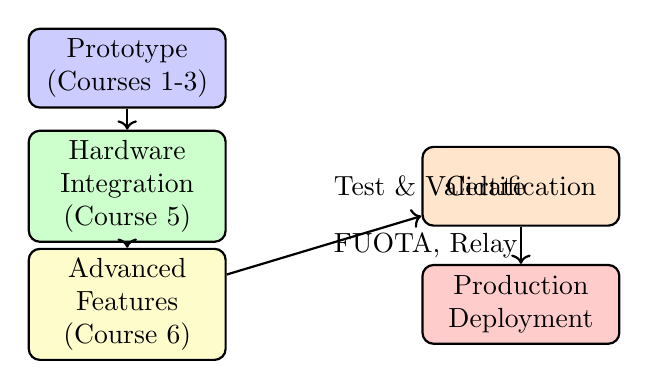
\begin{tikzpicture}[
    node distance=1.5cm,
    box/.style={rectangle, rounded corners, draw=black, thick, minimum height=1cm, minimum width=2.5cm, align=center}
]
    % Development stages
    \node[box, fill=blue!20] (proto) at (0,4) {Prototype\\(Courses 1-3)};
    \node[box, fill=green!20] (hw) at (0,2.5) {Hardware\\Integration\\(Course 5)};
    \node[box, fill=yellow!20] (features) at (0,1) {Advanced\\Features\\(Course 6)};
    \node[box, fill=orange!20] (cert) at (5,2.5) {Certification};
    \node[box, fill=red!20] (prod) at (5,1) {Production\\Deployment};

    % Arrows
    \draw[->, thick] (proto) -- (hw);
    \draw[->, thick] (hw) -- (features);
    \draw[->, thick] (features) -- (cert);
    \draw[->, thick] (cert) -- (prod);

    % Labels
    \node[right] at (2.5,2.5) {Test \& Validate};
    \node[right] at (2.5,1.75) {FUOTA, Relay};
\end{tikzpicture}
\end{center}
\end{frame}

% ============================================================================
\section{FUOTA (Firmware Update Over-The-Air)}
% ============================================================================

\begin{frame}{What is FUOTA?}
\begin{block}{Definition}
FUOTA (Firmware Update Over-The-Air) enables remote firmware updates for LoRaWAN devices without physical access.
\end{block}

\vspace{0.3cm}

\textbf{Key Benefits:}
\begin{itemize}
    \item Update deployed devices remotely
    \item Fix bugs without device retrieval
    \item Add new features post-deployment
    \item Reduce maintenance costs
    \item Extend device lifetime
\end{itemize}

\vspace{0.3cm}

\textbf{Use Cases:}
\begin{itemize}
    \item Smart city sensors (thousands of devices)
    \item Remote agricultural monitoring
    \item Industrial IoT in hazardous locations
    \item Underground or underwater deployments
\end{itemize}
\end{frame}

\begin{frame}{FUOTA Architecture}
\begin{center}
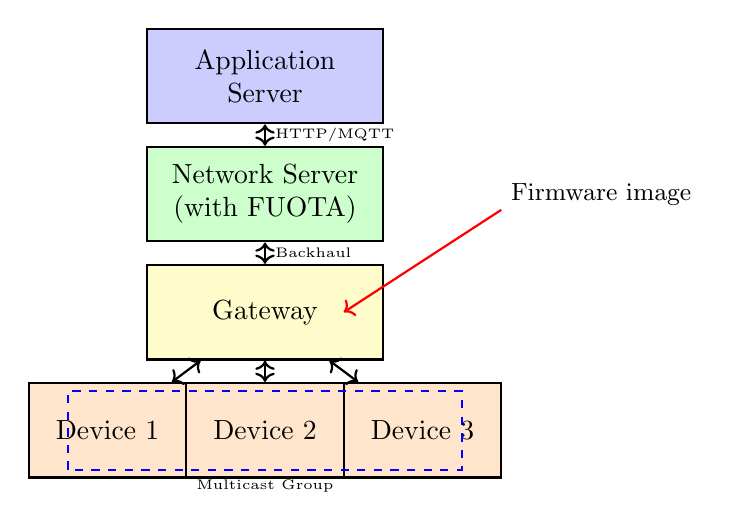
\begin{tikzpicture}[
    node distance=2cm,
    box/.style={rectangle, draw=black, thick, minimum height=1.2cm, minimum width=3cm, align=center}
]
    % Application Server
    \node[box, fill=blue!20] (as) at (0,4) {Application\\Server};

    % Network Server
    \node[box, fill=green!20] (ns) at (0,2.5) {Network Server\\(with FUOTA)};

    % Gateway
    \node[box, fill=yellow!20] (gw) at (0,1) {Gateway};

    % End Devices
    \node[box, fill=orange!20, minimum width=2cm] (ed1) at (-2,-0.5) {Device 1};
    \node[box, fill=orange!20, minimum width=2cm] (ed2) at (0,-0.5) {Device 2};
    \node[box, fill=orange!20, minimum width=2cm] (ed3) at (2,-0.5) {Device 3};

    % Connections
    \draw[<->, thick] (as) -- (ns) node[midway, right] {\tiny HTTP/MQTT};
    \draw[<->, thick] (ns) -- (gw) node[midway, right] {\tiny Backhaul};
    \draw[<->, thick] (gw) -- (ed1);
    \draw[<->, thick] (gw) -- (ed2);
    \draw[<->, thick] (gw) -- (ed3);

    % Firmware annotation
    \node[right] at (3,2.5) {\small Firmware image};
    \draw[->, thick, red] (3,2.3) -- (1,1);

    % Multicast group
    \draw[dashed, thick, blue] (-2.5,-1) rectangle (2.5,0);
    \node[below] at (0,-1) {\tiny Multicast Group};
\end{tikzpicture}
\end{center}
\end{frame}

\begin{frame}{FUOTA Process Flow}
\begin{enumerate}
    \item \textbf{Setup Multicast Session}
    \begin{itemize}
        \item Network Server creates multicast group
        \item Devices join multicast session
        \item Session keys distributed
    \end{itemize}

    \item \textbf{Firmware Fragmentation}
    \begin{itemize}
        \item Firmware split into fragments (typ. 200 bytes each)
        \item Reed-Solomon FEC (Forward Error Correction)
        \item Redundancy for lost packets
    \end{itemize}

    \item \textbf{Multicast Transmission}
    \begin{itemize}
        \item Network Server broadcasts fragments
        \item Devices collect fragments
        \item Request missing fragments (unicast)
    \end{itemize}

    \item \textbf{Validation and Installation}
    \begin{itemize}
        \item Verify firmware integrity (CRC, signature)
        \item Install to secondary slot (MCUboot)
        \item Reboot and swap images
    \end{itemize}
\end{enumerate}
\end{frame}

\begin{frame}{FUOTA Fragmentation}
\begin{center}
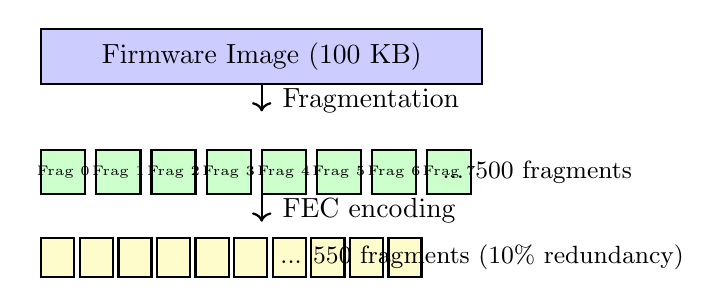
\begin{tikzpicture}[scale=0.7]
    % Firmware image
    \draw[thick, fill=blue!20] (0,3) rectangle (8,4);
    \node at (4,3.5) {Firmware Image (100 KB)};

    % Arrow down
    \draw[->, thick] (4,3) -- (4,2.5);
    \node[right] at (4.2,2.7) {Fragmentation};

    % Fragments
    \foreach \x in {0,1,2,3,4,5,6,7} {
        \draw[thick, fill=green!20] (\x,1) rectangle (\x+0.8,1.8);
        \node at (\x+0.4,1.4) {\tiny Frag \x};
    }
    \node at (9,1.4) {\small ... 500 fragments};

    % Arrow down
    \draw[->, thick] (4,1) -- (4,0.5);
    \node[right] at (4.2,0.7) {FEC encoding};

    % Encoded fragments with redundancy
    \foreach \x in {0,1,2,3,4,5,6,7,8,9} {
        \pgfmathsetmacro{\xpos}{\x*0.7}
        \draw[thick, fill=yellow!20] (\xpos,-0.5) rectangle (\xpos+0.6,0.2);
    }
    \node at (8,-0.15) {\small ... 550 fragments (10\% redundancy)};
\end{tikzpicture}
\end{center}

\vspace{0.3cm}

\textbf{Fragment Size:} 200 bytes typical (fits in LoRaWAN payload)\\
\textbf{Redundancy:} 5-10\% extra fragments for error correction\\
\textbf{Time Estimate:} 100 KB firmware, 500 fragments, 1 per minute = 8 hours
\end{frame}

\begin{frame}[fragile]{FUOTA Implementation with LBM}
\begin{lstlisting}[caption={Enable FUOTA in LBM}]
#include <smtc_modem_api.h>

void fuota_init(void) {
    // Enable multicast
    smtc_modem_multicast_set_grp_config(
        0,  // Stack ID
        0,  // Multicast group index
        MULTICAST_ADDR,
        MULTICAST_NWK_SKEY,
        MULTICAST_APP_SKEY
    );

    // Configure firmware update service
    smtc_modem_file_upload_init(0, CIPHER_MODE_AES_CCM);

    // Set firmware size
    smtc_modem_stream_init(0, FW_SIZE,
                           STREAM_ENCRYPTION_ENABLE);

    printk("FUOTA initialized\n");
}
\end{lstlisting}
\end{frame}

\begin{frame}[fragile]{FUOTA Event Handling}
\begin{lstlisting}[caption={Handle FUOTA Events}]
void fuota_event_handler(void) {
    smtc_modem_event_t event;

    while (smtc_modem_get_event(&event, &pending)
           == SMTC_MODEM_RC_OK) {
        switch (event.event_type) {
        case SMTC_MODEM_EVENT_STREAM_DONE:
            printk("Firmware download complete!\n");
            verify_and_install_firmware();
            break;

        case SMTC_MODEM_EVENT_UPLOAD_DONE:
            printk("Upload session complete\n");
            break;

        case SMTC_MODEM_EVENT_FIRMWARE_MANAGEMENT:
            handle_firmware_management(&event);
            break;
        }
    }
}
\end{lstlisting}
\end{frame}

\begin{frame}[fragile]{MCUboot Integration}
\begin{lstlisting}[caption={Install Downloaded Firmware}]
#include <zephyr/dfu/mcuboot.h>
#include <zephyr/storage/flash_map.h>

void verify_and_install_firmware(void) {
    // Verify firmware signature
    if (!verify_firmware_signature()) {
        printk("Firmware signature invalid!\n");
        return;
    }

    // Mark image as pending (MCUboot will swap)
    int ret = boot_request_upgrade(
        BOOT_UPGRADE_TEST);

    if (ret == 0) {
        printk("Firmware marked for upgrade\n");
        printk("Rebooting in 5 seconds...\n");
        k_sleep(K_SECONDS(5));
        sys_reboot(SYS_REBOOT_WARM);
    } else {
        printk("Failed to mark upgrade: %d\n", ret);
    }
}
\end{lstlisting}
\end{frame}

\begin{frame}{FUOTA Best Practices}
\begin{block}{Design Considerations}
\begin{itemize}
    \item \textbf{Image Size:} Keep firmware < 200 KB to reduce update time
    \item \textbf{Timing:} Schedule updates during low-traffic periods
    \item \textbf{Redundancy:} Use 10\% FEC redundancy for reliable transfer
    \item \textbf{Verification:} Always verify signature before installation
    \item \textbf{Rollback:} Implement fallback to previous firmware if update fails
\end{itemize}
\end{block}

\vspace{0.3cm}

\begin{alertblock}{Security}
\begin{itemize}
    \item Use cryptographic signatures (Ed25519 or ECDSA)
    \item Encrypt firmware images
    \item Validate firmware before installation
    \item Protect firmware download from tampering
\end{itemize}
\end{alertblock}
\end{frame}

% ============================================================================
\section{LoRaWAN Relay}
% ============================================================================

\begin{frame}{LoRaWAN Relay Overview}
\begin{block}{What is LoRaWAN Relay?}
LoRaWAN Relay extends network coverage by allowing end devices to relay packets from other devices.
\end{block}

\vspace{0.3cm}

\textbf{Use Cases:}
\begin{itemize}
    \item Extend coverage in buildings (indoor to outdoor)
    \item Bridge gaps in network coverage (dead zones)
    \item Reach devices in basements or tunnels
    \item Reduce gateway infrastructure costs
\end{itemize}

\vspace{0.3cm}

\textbf{Two Modes:}
\begin{itemize}
    \item \textbf{Served End Device:} Device with poor coverage (needs relay)
    \item \textbf{Relay Device:} Device with good coverage (provides relay)
\end{itemize}
\end{frame}

\begin{frame}{Relay Network Topology}
\begin{center}
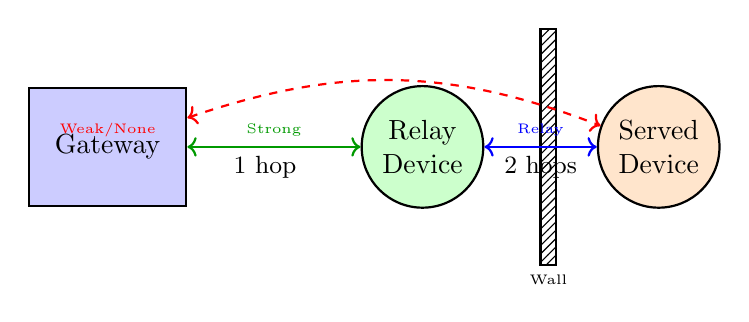
\begin{tikzpicture}[
    node distance=2cm,
    device/.style={circle, draw=black, thick, minimum size=1.2cm, align=center},
    gateway/.style={rectangle, draw=black, thick, minimum height=1.5cm, minimum width=2cm, align=center}
]
    % Gateway
    \node[gateway, fill=blue!20] (gw) at (0,0) {Gateway};

    % Relay device (good coverage)
    \node[device, fill=green!20] (relay) at (4,0) {Relay\\Device};

    % Served device (poor coverage, behind wall)
    \node[device, fill=orange!20] (served) at (7,0) {Served\\Device};

    % Wall
    \draw[thick, pattern=north east lines] (5.5,-1.5) rectangle (5.7,1.5);
    \node[below] at (5.6,-1.5) {\tiny Wall};

    % Direct link (good signal)
    \draw[<->, thick, green!60!black] (gw) -- (relay) node[midway, above] {\tiny Strong};

    % Weak/no direct link
    \draw[<->, thick, red, dashed] (gw) to[bend left=20] (served) node[midway, above] {\tiny Weak/None};

    % Relay link (2-hop)
    \draw[<->, thick, blue] (relay) -- (served) node[midway, above] {\tiny Relay};

    % Annotations
    \node[below] at (2,0) {\small 1 hop};
    \node[below] at (5.5,0) {\small 2 hops};
\end{tikzpicture}
\end{center}

\vspace{0.3cm}

\textbf{Relay Benefits:}
\begin{itemize}
    \item Served device reaches gateway via relay (2-hop)
    \item No infrastructure changes needed
    \item Dynamic relay selection
\end{itemize}
\end{frame}

\begin{frame}{Relay Packet Flow}
\begin{center}
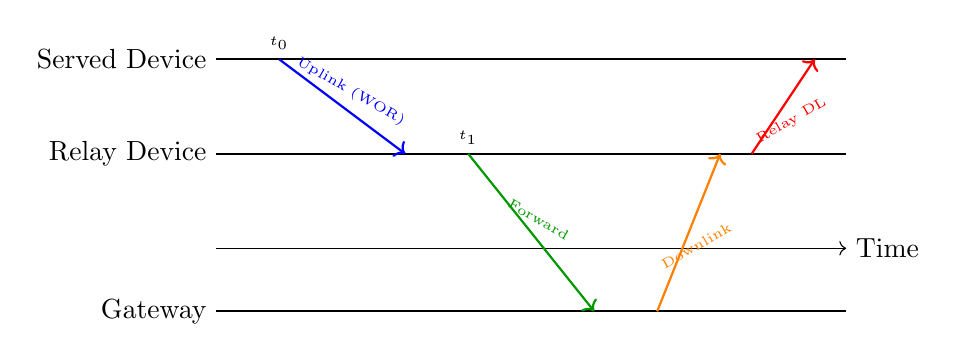
\begin{tikzpicture}[scale=0.8]
    % Timeline
    \draw[->] (0,0) -- (10,0) node[right] {Time};

    % Actors
    \draw[thick] (0,3) -- (10,3);
    \node[left] at (0,3) {Served Device};

    \draw[thick] (0,1.5) -- (10,1.5);
    \node[left] at (0,1.5) {Relay Device};

    \draw[thick] (0,-1) -- (10,-1);
    \node[left] at (0,-1) {Gateway};

    % Step 1: Served device transmits on WOR channel
    \draw[->, thick, blue] (1,3) -- (3,1.5) node[midway, above, rotate=-30] {\tiny Uplink (WOR)};
    \node[above] at (1,3) {\tiny $t_0$};

    % Step 2: Relay receives and forwards
    \draw[->, thick, green!60!black] (4,1.5) -- (6,-1) node[midway, above, rotate=-30] {\tiny Forward};
    \node[above] at (4,1.5) {\tiny $t_1$};

    % Step 3: Gateway sends downlink to relay
    \draw[->, thick, orange] (7,-1) -- (8,1.5) node[midway, below, rotate=30] {\tiny Downlink};

    % Step 4: Relay forwards to served device
    \draw[->, thick, red] (8.5,1.5) -- (9.5,3) node[midway, below, rotate=30] {\tiny Relay DL};
\end{tikzpicture}
\end{center}

\vspace{0.3cm}

\textbf{Key Concepts:}
\begin{itemize}
    \item \textbf{WOR (Wake-On-Radio):} Low-power preamble detection
    \item \textbf{CAD (Channel Activity Detection):} Relay listens for preambles
    \item \textbf{Forwarding:} Relay re-transmits packet to gateway
\end{itemize}
\end{frame}

\begin{frame}[fragile]{Configure Relay Mode - Served Device}
\begin{lstlisting}[caption={Enable Relay for Served Device}]
#include <smtc_modem_api.h>
#include <smtc_modem_relay_api.h>

void relay_served_init(void) {
    // Enable relay mode
    smtc_modem_relay_tx_enable(0, true);

    // Configure WOR settings
    smtc_modem_relay_tx_set_activation_mode(
        0, SMTC_MODEM_RELAY_TX_ACTIVATION_MODE_ED);

    // Set relay search period
    smtc_modem_relay_tx_set_smart_level(0, 8);

    // Use WOR channel for uplinks
    smtc_modem_relay_tx_set_backoff(0, 60);  // 60s

    printk("Relay served mode enabled\n");
}
\end{lstlisting}
\end{frame}

\begin{frame}[fragile]{Configure Relay Mode - Relay Device}
\begin{lstlisting}[caption={Enable Relay Forwarding}]
void relay_device_init(void) {
    // Enable relay RX mode (forwarding)
    smtc_modem_relay_rx_enable(0, true);

    // Configure relay behavior
    smtc_modem_relay_rx_set_activation_mode(
        0, SMTC_MODEM_RELAY_RX_ACTIVATION_MODE_ENABLE);

    // Set forwarding rules
    smtc_modem_relay_rx_set_smart_level(0, 8);

    // CAD period (wake to listen for WOR)
    smtc_modem_relay_rx_set_backoff(0, 60);  // 60s

    printk("Relay device mode enabled\n");
}

void relay_event_handler(void) {
    if (event.event_type ==
        SMTC_MODEM_EVENT_RELAY_TX_DYNAMIC) {
        printk("Forwarded packet for served device\n");
    }
}
\end{lstlisting}
\end{frame}

\begin{frame}{Relay Power Consumption}
\begin{block}{Challenge}
Relay devices must wake periodically to detect WOR preambles, increasing power consumption.
\end{block}

\vspace{0.3cm}

\textbf{Optimization Strategies:}
\begin{itemize}
    \item \textbf{Adaptive CAD:} Increase CAD period when no traffic
    \item \textbf{Smart Level:} Adjust relay sensitivity based on RSSI
    \item \textbf{Battery vs. Mains:} Use mains-powered devices as relays
    \item \textbf{Duty Cycling:} Enable relay only during certain hours
\end{itemize}

\vspace{0.3cm}

\textbf{Typical Current:}
\begin{itemize}
    \item Normal operation: 5 µA sleep
    \item With relay (CAD every 60s): 20 µA average
    \item 4x increase in power consumption
\end{itemize}

\begin{alertblock}{Recommendation}
Use mains-powered or solar-powered devices as relays whenever possible.
\end{alertblock}
\end{frame}

% ============================================================================
\section{LoRaWAN Certification}
% ============================================================================

\begin{frame}{Why LoRaWAN Certification?}
\begin{block}{Certification Benefits}
\begin{itemize}
    \item Guarantees interoperability with all LoRaWAN networks
    \item Required by many operators and customers
    \item Demonstrates compliance with LoRaWAN specification
    \item Builds trust and credibility
    \item Access to LoRa Alliance logo and marketing
\end{itemize}
\end{block}

\vspace{0.3cm}

\textbf{Certification Levels:}
\begin{itemize}
    \item \textbf{Pre-Certification:} Self-testing with open tools
    \item \textbf{Official Certification:} Third-party lab testing
    \item \textbf{Re-Certification:} After major firmware changes
\end{itemize}

\vspace{0.3cm}

\textbf{Certification Cost:} Typically \$2,000 - \$5,000 USD per device type
\end{frame}

\begin{frame}{Certification Test Categories}
\begin{enumerate}
    \item \textbf{MAC Layer Compliance}
    \begin{itemize}
        \item OTAA join procedure
        \item Uplink/downlink handling
        \item Adaptive Data Rate (ADR)
        \item RX windows timing
        \item Duty cycle compliance
    \end{itemize}

    \item \textbf{PHY Layer Compliance}
    \begin{itemize}
        \item Frequency accuracy (±20 ppm)
        \item TX power accuracy
        \item Modulation parameters
        \item Receive sensitivity
    \end{itemize}

    \item \textbf{Regional Parameters}
    \begin{itemize}
        \item EU868, US915, AS923, etc.
        \item Channel plans
        \item Duty cycle limits
        \item Dwell time limits
    \end{itemize}
\end{enumerate}
\end{frame}

\begin{frame}{Certification Testing Setup}
\begin{center}
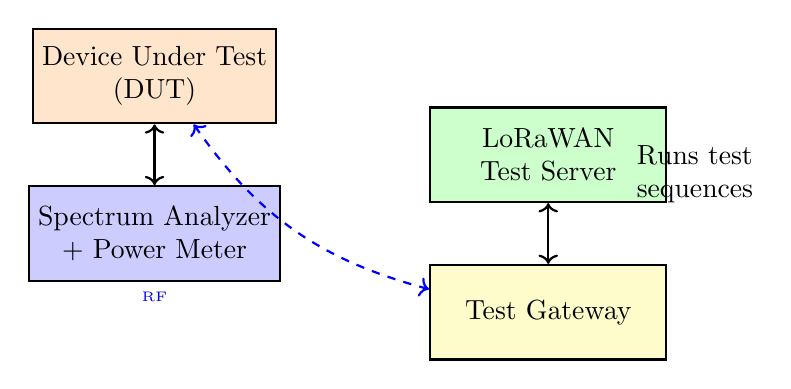
\begin{tikzpicture}[
    box/.style={rectangle, draw=black, thick, minimum height=1.2cm, minimum width=3cm, align=center}
]
    % DUT
    \node[box, fill=orange!20] (dut) at (0,3) {Device Under Test\\(DUT)};

    % Test equipment
    \node[box, fill=blue!20] (analyzer) at (0,1) {Spectrum Analyzer\\+ Power Meter};

    % Test server
    \node[box, fill=green!20] (server) at (5,2) {LoRaWAN\\Test Server};

    % Gateway
    \node[box, fill=yellow!20] (gw) at (5,0) {Test Gateway};

    % Connections
    \draw[<->, thick] (dut) -- (analyzer);
    \draw[<->, thick, dashed, blue] (dut) to[bend right=20] (gw) node[midway, above] {\tiny RF};
    \draw[<->, thick] (gw) -- (server);

    % Annotations
    \node[right] at (6,2) {Runs test};
    \node[right] at (6,1.5) {sequences};
\end{tikzpicture}
\end{center}

\vspace{0.3cm}

\textbf{Test Tools:}
\begin{itemize}
    \item LoRa Alliance Test Tool (official)
    \item End Device Certification Test Suite
    \item RF test equipment (spectrum analyzer, power meter)
\end{itemize}
\end{frame}

\begin{frame}{Common Certification Failures}
\begin{block}{1. RX Window Timing}
\textbf{Issue:} RX1/RX2 windows not opened at correct time\\
\textbf{Fix:} Calibrate crystal, improve timing accuracy
\end{block}

\begin{block}{2. Duty Cycle Violation}
\textbf{Issue:} Exceeds 1\% (EU) or dwell time limits\\
\textbf{Fix:} Implement proper duty cycle tracking
\end{block}

\begin{block}{3. TX Power Inaccuracy}
\textbf{Issue:} Actual TX power differs from configured\\
\textbf{Fix:} Calibrate TX power (see Course 5)
\end{block}

\begin{block}{4. ADR Not Working}
\textbf{Issue:} Device doesn't respond to ADR commands\\
\textbf{Fix:} Enable ADR in LBM, test with varying RSSI
\end{block}
\end{frame}

\begin{frame}[fragile]{Prepare for Certification}
\begin{lstlisting}[caption={Enable All LoRaWAN Features}]
// prj.conf - Enable certification features

CONFIG_LORAWAN_VERSION_1_0_4=y
CONFIG_LORAWAN_DUTYCYCLE=y
CONFIG_LORAWAN_ADR=y
CONFIG_LORAWAN_PUBLIC_NETWORK=y

// Enable all supported regions
CONFIG_LORAWAN_REGION_EU868=y
CONFIG_LORAWAN_REGION_US915=y
CONFIG_LORAWAN_REGION_AS923=y

// Enable class B/C if supported
CONFIG_LORAWAN_CLASS_B=y
CONFIG_LORAWAN_CLASS_C=y

// Enable proper NVM for persistent storage
CONFIG_NVS=y
CONFIG_LORAWAN_NVM_CONTEXT_MGMT=y
\end{lstlisting}
\end{frame}

% ============================================================================
\section{Production Optimization}
% ============================================================================

\begin{frame}{Production Checklist}
\begin{enumerate}
    \item \textbf{Security}
    \begin{itemize}
        \item Unique DevEUI, JoinEUI, AppKey per device
        \item Secure key storage (e.g., secure element)
        \item Encrypted firmware images
        \item Disable debug interfaces
    \end{itemize}

    \item \textbf{Power Optimization}
    \begin{itemize}
        \item Enable low-power modes (Course 2)
        \item Optimize uplink interval
        \item Use confirmed uplinks sparingly
        \item Implement adaptive strategies
    \end{itemize}

    \item \textbf{Reliability}
    \begin{itemize}
        \item Implement watchdog timer
        \item Handle join failures gracefully
        \item Store critical data in NVM
        \item Test in real-world conditions
    \end{itemize}
\end{enumerate}
\end{frame}

\begin{frame}{Security Best Practices}
\begin{alertblock}{CRITICAL: Unique Keys}
Every device MUST have unique:
\begin{itemize}
    \item DevEUI (globally unique 64-bit ID)
    \item JoinEUI (formerly AppEUI)
    \item AppKey (128-bit secret key)
\end{itemize}
\textbf{Never} reuse keys across devices!
\end{alertblock}

\vspace{0.3cm}

\textbf{Key Provisioning Options:}
\begin{enumerate}
    \item \textbf{Pre-Provisioned:} Keys programmed during manufacturing
    \item \textbf{Secure Element:} Keys stored in ATECC608 or similar
    \item \textbf{On-Demand:} Keys generated and assigned during commissioning
\end{enumerate}

\vspace{0.3cm}

\textbf{Protect Keys:}
\begin{itemize}
    \item Store in flash with read-out protection
    \item Use MPU/TrustZone if available
    \item Disable JTAG/SWD in production
\end{itemize}
\end{frame}

\begin{frame}[fragile]{Provision Unique Keys}
\begin{lstlisting}[caption={Key Provisioning Example}]
// Read DevEUI from secure storage or MCU unique ID
void get_device_eui(uint8_t *dev_eui) {
    // Option 1: Use MCU unique ID
    uint32_t *uid = (uint32_t *)0x0FE081F0;  // nRF54L15
    memcpy(dev_eui, uid, 8);

    // Option 2: Read from secure element
    // atecc608_read_serial(dev_eui);

    // Option 3: Read from provisioned flash region
    // flash_read(PROVISIONING_ADDR, dev_eui, 8);
}

void lorawan_provision(void) {
    uint8_t dev_eui[8];
    uint8_t join_eui[8] = LORAWAN_JOIN_EUI;
    uint8_t app_key[16] = LORAWAN_APP_KEY;

    get_device_eui(dev_eui);

    smtc_modem_set_deveui(0, dev_eui);
    smtc_modem_set_joineui(0, join_eui);
    smtc_modem_set_nwkkey(0, app_key);
}
\end{lstlisting}
\end{frame}

\begin{frame}{Manufacturing Test Flow}
\begin{center}
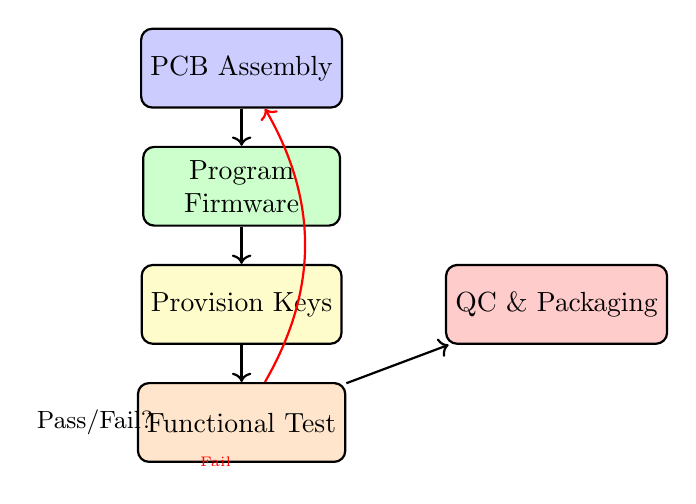
\begin{tikzpicture}[
    node distance=1.5cm,
    box/.style={rectangle, rounded corners, draw=black, thick, minimum height=1cm, minimum width=2.5cm, align=center}
]
    % Manufacturing steps
    \node[box, fill=blue!20] (pcb) at (0,5) {PCB Assembly};
    \node[box, fill=green!20] (program) at (0,3.5) {Program\\Firmware};
    \node[box, fill=yellow!20] (provision) at (0,2) {Provision Keys};
    \node[box, fill=orange!20] (test) at (0,0.5) {Functional Test};
    \node[box, fill=red!20] (qc) at (4,2) {QC \& Packaging};

    % Arrows
    \draw[->, thick] (pcb) -- (program);
    \draw[->, thick] (program) -- (provision);
    \draw[->, thick] (provision) -- (test);
    \draw[->, thick] (test) -- (qc);

    % Test results
    \node[left] at (-1,0.5) {\small Pass/Fail?};
    \draw[->, thick, red] (test) to[bend right=30] (pcb) node[midway, left] {\tiny Fail};
\end{tikzpicture}
\end{center}

\vspace{0.3cm}

\textbf{Functional Tests:}
\begin{itemize}
    \item Read chip ID (verify communication)
    \item Perform LoRaWAN join
    \item Send test uplink
    \item Measure TX power (spot check)
    \item Verify GPS/sensor readings
\end{itemize}
\end{frame}

\begin{frame}{Field Deployment Considerations}
\begin{columns}
\column{0.5\textwidth}
\textbf{Environmental:}
\begin{itemize}
    \item IP67/IP68 enclosure
    \item Operating temp range
    \item UV resistance
    \item Moisture protection
    \item Vibration tolerance
\end{itemize}

\vspace{0.3cm}

\textbf{Antenna:}
\begin{itemize}
    \item External vs. internal
    \item Vertical polarization
    \item Ground plane requirements
    \item Avoid metal enclosures
\end{itemize}

\column{0.5\textwidth}
\textbf{Battery:}
\begin{itemize}
    \item Li-SOCI$_2$ for long life
    \item LiPo for rechargeable
    \item Capacity calculation
    \item Temperature derating
\end{itemize}

\vspace{0.3cm}

\textbf{Installation:}
\begin{itemize}
    \item Outdoor mounting
    \item Line-of-sight to gateway
    \item Avoid Faraday cages
    \item Test coverage before install
    \item Document GPS coordinates
\end{itemize}
\end{columns}
\end{frame}

% ============================================================================
\section{Hands-On Labs}
% ============================================================================

\begin{frame}{Lab 6.1: FUOTA Implementation}
\begin{block}{Objective}
Implement firmware update over-the-air using multicast and LBM.
\end{block}

\textbf{Tasks:}
\begin{enumerate}
    \item Enable MCUboot bootloader with dual-image support
    \item Configure LBM for multicast and file upload
    \item Join LoRaWAN network
    \item Configure network server to send firmware update
    \item Receive firmware fragments via multicast
    \item Verify and install updated firmware
    \item Test rollback if update fails
\end{enumerate}

\vspace{0.3cm}

\textbf{Deliverables:}
\begin{itemize}
    \item FUOTA-enabled firmware
    \item Successful OTA update demonstration
    \item Serial logs showing update process
\end{itemize}
\end{frame}

\begin{frame}{Lab 6.2: LoRaWAN Relay Configuration}
\begin{block}{Objective}
Configure one device as relay and another as served device to extend coverage.
\end{block}

\textbf{Tasks:}
\begin{enumerate}
    \item Configure Device A as relay device (good coverage location)
    \item Configure Device B as served device (poor coverage location)
    \item Test direct uplink from Device B (expect failure/weak signal)
    \item Enable relay mode on both devices
    \item Test uplink from Device B via relay (expect success)
    \item Monitor relay events and packet forwarding
    \item Measure additional power consumption on relay device
\end{enumerate}

\vspace{0.3cm}

\textbf{Deliverables:}
\begin{itemize}
    \item Relay and served device firmware
    \item Coverage comparison (with/without relay)
    \item Power consumption analysis
\end{itemize}
\end{frame}

\begin{frame}{Lab 6.3: Certification Pre-Testing}
\begin{block}{Objective}
Perform self-testing to prepare for official LoRaWAN certification.
\end{block}

\textbf{Tasks:}
\begin{enumerate}
    \item Download LoRa Alliance End Device Test Tool
    \item Set up local LoRaWAN test network
    \item Run MAC compliance tests (OTAA, ADR, duty cycle)
    \item Run PHY compliance tests (frequency, power, sensitivity)
    \item Run regional parameter tests (EU868 or US915)
    \item Document any failures and fix issues
    \item Re-test until all tests pass
\end{enumerate}

\vspace{0.3cm}

\textbf{Deliverables:}
\begin{itemize}
    \item Test results report
    \item List of issues found and fixes applied
    \item Final passing test results
\end{itemize}
\end{frame}

\begin{frame}{Lab 6.4: Production Optimization}
\begin{block}{Objective}
Optimize firmware for production deployment with security and power savings.
\end{block}

\textbf{Tasks:}
\begin{enumerate}
    \item Implement unique key provisioning from MCU UID
    \item Enable secure boot and flash read-out protection
    \item Optimize power consumption (target < 10 µA average)
    \item Add watchdog timer and error recovery
    \item Implement persistent storage for critical state
    \item Create manufacturing test firmware
    \item Measure battery life estimate (with profiler)
\end{enumerate}

\vspace{0.3cm}

\textbf{Deliverables:}
\begin{itemize}
    \item Production-ready firmware
    \item Power consumption report
    \item Battery life calculation
    \item Manufacturing test procedure
\end{itemize}
\end{frame}

% ============================================================================
\section{Summary}
% ============================================================================

\begin{frame}{Course 6 Summary}
\begin{block}{Key Takeaways}
\begin{itemize}
    \item FUOTA enables remote firmware updates for deployed devices
    \item LoRaWAN Relay extends coverage without additional infrastructure
    \item Certification ensures interoperability and compliance
    \item Production requires unique keys, security, and optimization
    \item Real-world deployment needs environmental and RF considerations
\end{itemize}
\end{block}

\vspace{0.5cm}

\textbf{Congratulations!}
\begin{itemize}
    \item You've completed all 6 USP training courses
    \item You're ready to develop production LoRaWAN devices
    \item Continue learning with advanced topics and certifications
\end{itemize}
\end{frame}

\begin{frame}{Training Series Complete}
\begin{center}
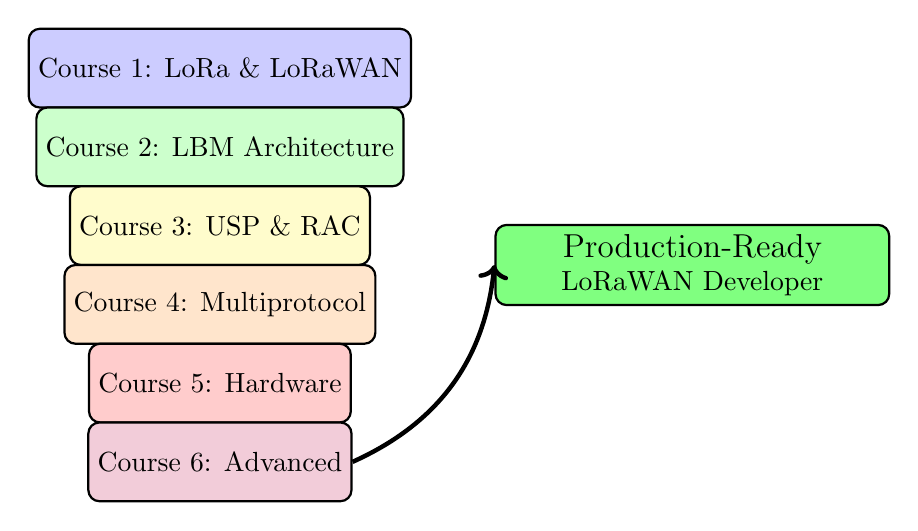
\begin{tikzpicture}[
    box/.style={rectangle, rounded corners, draw=black, thick, minimum height=1cm, minimum width=3cm, align=center}
]
    % All courses
    \node[box, fill=blue!20] (c1) at (0,5) {Course 1: LoRa \& LoRaWAN};
    \node[box, fill=green!20] (c2) at (0,4) {Course 2: LBM Architecture};
    \node[box, fill=yellow!20] (c3) at (0,3) {Course 3: USP \& RAC};
    \node[box, fill=orange!20] (c4) at (0,2) {Course 4: Multiprotocol};
    \node[box, fill=red!20] (c5) at (0,1) {Course 5: Hardware};
    \node[box, fill=purple!20] (c6) at (0,0) {Course 6: Advanced};

    % Outcome
    \node[box, fill=green!50, minimum width=5cm] (outcome) at (6,2.5) {\large Production-Ready\\LoRaWAN Developer};

    % Arrow
    \draw[->, ultra thick] (c6.east) to[bend right=30] (outcome.west);
\end{tikzpicture}
\end{center}
\end{frame}

\begin{frame}{Additional Resources}
\textbf{Documentation:}
\begin{itemize}
    \item LoRa Alliance Specifications: 
    \item LBM Documentation: 
    \item Zephyr RTOS Docs: 
    \item MCUboot: 
\end{itemize}

\vspace{0.3cm}

\textbf{Certification:}
\begin{itemize}
    \item LoRa Alliance Device Certification: 
    \item End Device Test Tool
\end{itemize}

\vspace{0.3cm}

\textbf{Community:}
\begin{itemize}
    \item LoRa Alliance Technical Committee
    \item The Things Network Community
    \item Zephyr Discord
\end{itemize}
\end{frame}

\begin{frame}[plain]
\begin{center}
\Huge Thank You!

\vspace{1cm}

\Large Congratulations on Completing\\USP Training Series

\vspace{1cm}

\normalsize
\textbf{Questions or Support:}\\
\texttt{usp-support@example.com}

\vspace{0.5cm}

\textbf{Lab Solutions:}\\
\texttt{doc/training/Lab\_Solutions.md}
\end{center}
\end{frame}

\end{document}
